\subsection{Lottery Scheduling}

La idea detr\'as de $lottery$ $scheduling$\cite{SchedLottery} es aplicar un enfoque probabil\'istico y pseudoaleatorio a la hora de asignar recursos a las tareas. Para lograr esto se utiliza un sistema de $tickets$ que representan derechos de acceso a recursos; las tareas poseen una cantidad determinada de $tickets$, puediendo ser distinta de una tarea a otra y cada vez que el $scheduler$ decide a qu\'e tarea otorgar los recursos lo hace mediante una loter\'ia, elige uno entre todos los $tickets$ del sistema. El proceso que tenga ese $ticket$ ser\'a el ganador y se le asignar\'a el recurso que est\'a demandado.

Los $tickets$ son una forma de cuantificar los derechos de acceso a recursos; cuantos m\'as $tickets$ tenga una tarea, m\'as probable es que gane la loter\'ia. Tambi\'en permiten homogeneizar los diferentes tipos de recursos ya que todos son representados por los mismos tipos de $tickets$, esto aporta flexibilidad a la hora de asignarlos.

\subsubsection{Loter\'ias}

En cada $tick$ del reloj, el $scheduler$ toma una decisi\'on: si el proceso en ejecuci\'on agot\'o todo su quantum asignado, realiz\'o una llamada bloqueante o simplemente termin\'o exitosamente entonces se lleva a cabo una loter\'ia. Est\'a loter\'ia decide qui\'en va a ser el pr\'oximo proceso en utilizar el recurso deseado. Elegir el $ticket$ ganador se realiza mediante un algoritmo pseudoaleatorio que lo elige de manera uniforme, esto es, todos los tickets tienen una probabilidad igual de ganar la loter\'ia, a saber:

Sea $n$ la cantidad de $tickets$ y \{t$_i$\}$_{1 \leq i \leq n}$ el conjunto de ellos.

\[
	P(t_{i}) = \frac{1}{n}
\]

Luego, la probabilidad que un proceso $j$ que posee $t$ cantidad de $tickets$ gane la loter\'ia es igual a:


\[
	P(j \text{ gane la loter\'ia}) = \sum_{1}^{t}\frac{1}{n} = \frac{t}{n}
\]

Se puede probar que la cantidad de loter\'ias ganadas por la tarea $j$ sigue una distribuci\'on binomial de par\'ametro $p = \frac{t}{n}$. De esta manera se observa que la esperanza de la cantidad de loter\'ias ganadas por una tarea es igual a:

\[
	E(\text{cantidad de loter\'ias ganadas}) = \frac{t}{n}*\text{cantidad de loter\'ias realizadas}
\]

Esto implica que el valor promedio de la cantidad de loter\'ias ganadas es directamente proporcional a la cantidad de $tickets$ que posee la tarea. Por esta raz\'on se dice que $lottery$ $scheduling$ es probabil\'isticamente justo.

\subsubsection{Fairness}

\subsubsection{Compensation tickets}

Queremos ver cómo se comporta el algoritmo ante un lote de tareas compuesto por
tareas que sólo utilizan CPU y otras que realizan llamadas bloqueantes.\\

Si SchedLottery no contara con compensation tickets entonces como se explica en el artículo \cite[Sec. 3.4]{SchedLottery} el problema se 
ocasiona cuando una tarea se bloquea sin terminar de utilizar su quantum.
De continuar así por varios ciclos entonces esa tarea usaría, en promedio, menos CPU que las demás
(la probabilidad de ganar el sorteo es la misma para todas, pero en este caso habría tareas que
usan más tiempo el CPU que las demás)
violando así la regla de 1:1 dónde todas deberían recibir la misma proporción de CPU.\\

La forma propuesta para contrarrestar este problema es Compensation Tickets. 
Consiste en dar a la tarea bloqueada una cantidad de tickets en relación con el quantum no utilizado.
Así, si sólo utilizó una fracción $f$ del quantum le son dados $cant\_inicial/f$ tickets.\\

Queremos mostrar evidencia de que el sistema de compensation tickets (CT) corrige el problema
previamente mencionado sobre la asignación de CPU esperada entre tareas bloqueantes y no bloqueantes.
Para esto ejecutamos dos tareas, una taskBatch, ya que el problema se manifiesta cuando existen llamadas bloqueantes, y la otra taskCPU.\\

Al comienzo cada tarea posee 10 tickets (misma probabilidad de ganar) porque queremos que se ejecuten equitativamente.\\
Para mostrar que efectivamente hay una mejora en la distribución del CPU presentamos los datos mediante tablas, donde cada columna pertenece a un ciclo en particular 
y cada fila a una tarea.\\
Ej: La posición de la tabla fila x, columna y: tiene la cantidad de CPU utilizada por la tarea x hasta el ciclo y.\\

\begin{flushleft}
\textbf{SchedLottery sin CT:}\end{flushleft} %-------------------------------------------------------------------------------------------------------------

\begin{center}
 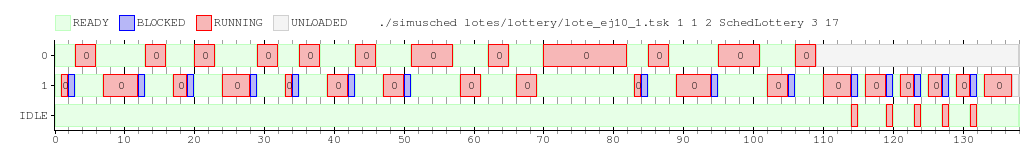
\includegraphics[scale=0.48]{./Lottery/ej10_SIN_CT.png}
\end{center}

\begin{center}
\begin{tabular}{|c|c|c|c|c|c|c|c|c|c|c|c|c|c|c|}
\hline
Ciclo & 10 & 20 & 30 & 40 & 50 & 60 & 70 & 80 & 90 & 100 & 110 & 120 & 130 & 137\\
\hline
\hline
Tarea 0 (CPU) & 3 & 6 & 10 & 15 & 18 & 24 & 27 & 37 & 42 & 47 & 51 & - & - & - \\
\hline
Tarea 1 (Batch) & 4 & 8 & 12 & 14 & 19 & 21 & 25 & 25 & 27 & 31 & 34 & 41 & 46 & 51 \\
\hline
\end{tabular}\end{center}

Hasta el ciclo 80 el CPU se mantiene relativamente distribuido. Luego la tarea 0 pasa a tener mayor proporción hasta que finaliza. 
Si esto se proyecta en el tiempo entonces la brecha se vuelve cada vez más grande.

\begin{flushleft}
\textbf{SchedLottery con CT:}\end{flushleft} %--------------------------------------------------------------------------------------------------------------

\begin{center}
 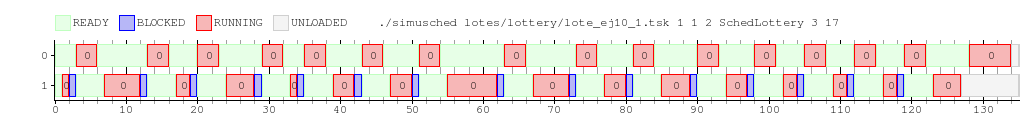
\includegraphics[scale=0.48]{./Lottery/ej10_CON_CT.png}
\end{center}

\begin{center}
\begin{tabular}{|c|c|c|c|c|c|c|c|c|c|c|c|c|c|c|}
\hline
Ciclo & 10 & 20 & 30 & 40 & 50 & 60 & 70 & 80 & 90 & 100 & 110 & 120 & 130 & 134 \\
\hline
\hline
Tarea 0 (CPU) & 3 & 6 & 10 & 15 & 18 & 21 & 24 & 27 & 30 & 35 & 39 & 43 & 47 & 51\\
\hline
Tarea 1 (Batch) & 4 & 8 & 12 & 14 & 19 & 24 & 29 & 34 & 38 & 41 & 44 & 47 & 51 & -\\
\hline
\end{tabular}\end{center}

